
\section{\pdfEinfty-coalgebras} \label{s:integrally}

An operad $\cO$ is said to be $E_\infty$ if there exists a morphism $\cO \to \com$ inducing in each arity $r$ a resolution of $\k$ by free $\k[\Sym_r]$-modules.

In this section we will describe the $E_\infty$-operad $\forget(\M)$ introduced in \cite{medina2020prop1} and use it to extend the natural coalgebra structures on simplicial and cubical chains to $E_\infty$-coalgebras.
Additionally, we will describe elements in this operad representing Steenord operations on the cohomology of these combinatorial models of spaces and overview the Brumfiel-Morgan program for algebraic Postnikov systems.

\subsection{Alexander--Whitney coalgebra} \label{ss:aw diagonal}

The first chain approximation to the diagonal was given in the simplicial context by \v{C}ech and Whitney building on independent work presented during the 1935 International Congress in Moscow by Alexander and Kolmogorov.
The original references are \cite{alexander1936ring, cech1936multiplication, whitney1938products} and a historical account is presented by Whitney in \cite[p.110]{whitney1988history}.
This chain map, referred to as the \textit{Alexander--Whitney coproduct}, is defined on canonical basis elements by the formula
\begin{equation} \label{e:alexander-whitney coalgebra}
\copr \big( [0,\dots,n] \big) = \sum_{i=0}^n \ [0, \dots, i] \ot [i, \dots, n].
\end{equation}
Together with the \textit{augmentation map}
\begin{equation} \label{e:augmentation map}
\aug \big( [0,\dots,n] \big) =
\begin{cases}
1 & n=0, \\ 0 & n=1,
\end{cases}
\end{equation}
the Alexander--Whitney coproduct satisfies
\begin{gather}
\label{e:coassociativity relation}
(\copr \ot \, \id) \circ \copr = (\id \ot \copr) \circ \copr, \\
\label{e:counital relation}
(\aug \ot \, \id) \circ \copr = \id = (\id \ot \aug) \circ \copr,
\end{gather}
making the chains of any simplicial set $X$ into a natural coassociative counital coalgebra, referred to as the \textit{Alexander--Whitney coalgebra} of $X$.

We will use the following recursively defined notation for general coalgebras:
\begin{align*}
\copr^1 &= \copr, \\
\copr^k &= (\copr \ot \, \id) \circ \copr^{k-1}.
\end{align*}

\subsection{The join product}

The \textit{join product} $\ast \colon \chains(\simplex^n)^{\ot 2} \to \chains(\simplex^n)$ is the natural degree~$1$ linear map defined by
\begin{multline}
\ast \big(\left[v_0, \dots, v_p \right] \ot \left[v_{p+1}, \dots, v_q\right]\big) = \\
\begin{cases} (-1)^{p} \sign(\pi) \left[v_{\pi(0)}, \dots, v_{\pi(q)}\right] & \text{ if } v_i \neq v_j \text{ for } i \neq j, \\
\hfil 0 & \text{ if not}, \end{cases}
\end{multline}
where $\pi$ is the permutation that orders the vertices.
It is an algebraic version of the usual join of faces in a simplex, please consult \cref{f:join of faces} for an example.

\begin{figure}
	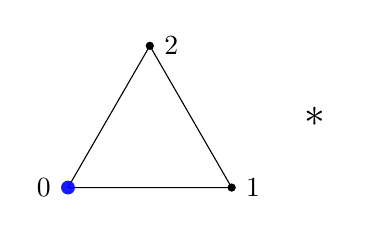
\begin{tikzpicture}[scale=.6]
\coordinate (A) at (210:2);
\coordinate (B) at (-30:2);
\coordinate (C) at (90:2);

\draw[draw=black] (A) -- (B) -- (C) -- (A);

\node[circle,fill=blue, opacity=.9, inner sep=0pt,minimum size=5pt, label=left:{0}] (a) at (A) {};
\node[circle,fill=black,inner sep=0pt,minimum size=3pt, label=right:{$1$}] (a) at (B) {};
\node[circle,fill=black,inner sep=0pt,minimum size=3pt, label=right:{$2$}] (a) at (C) {};

\node[scale=1.5] at (3.5,0.5) {$\ast$};
\end{tikzpicture}
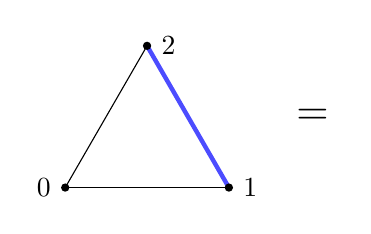
\begin{tikzpicture}[scale=.6]
\coordinate (A) at (210:2);
\coordinate (B) at (-30:2);
\coordinate (C) at (90:2);

\draw[draw=blue,  ultra thick, draw opacity=.7] (B) -- (C);
\draw[draw=black] (C) -- (A);
\draw[draw=black] (A) -- (B);

\node[circle,fill=black,inner sep=0pt,minimum size=3pt, label=left:{$0$}] (a) at (A) {};
\node[circle,fill=black,inner sep=0pt,minimum size=3pt, label=right:{$1$}] (a) at (B) {};
\node[circle,fill=black,inner sep=0pt,minimum size=3pt, label=right:{$2$}] (a) at (C) {};

\node[scale=1.5] at (3.5,.5) {=};
\end{tikzpicture}
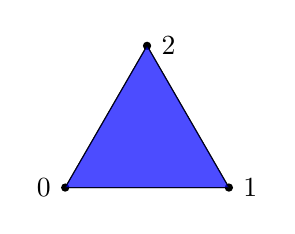
\begin{tikzpicture}[scale=.6]
\coordinate (A) at (210:2);
\coordinate (B) at (-30:2);
\coordinate (C) at (90:2);

\draw[draw=black] (A) -- (B) -- (C) -- (A);

\node[circle,fill=black,inner sep=0pt,minimum size=3pt, label=left:{$0$}] (a) at (A) {};
\node[circle,fill=black,inner sep=0pt,minimum size=3pt, label=right:{$1$}] (a) at (B) {};
\node[circle,fill=black,inner sep=0pt,minimum size=3pt, label=right:{$2$}] (a) at (C) {};

\draw[draw, fill=blue, opacity=.7] (A) -- (B) -- (C) -- (A);
\end{tikzpicture}
	\caption{Geometric representation of the join product of two basis elements. It depicts the identity $\pr \big( [0] \otimes [1,2] \big) = [0,1,2]$.}
	\label{f:join of faces}
\end{figure}

The join product can be used in conjunction with the Alexander--Whitney coproduct to canonically construct boundaries in the chain complexes
\[
\Hom \big( \chains(\simplex^n)^{\ot s}, \chains(\simplex^n)^{\ot r} \big).
\]
For example,
\[
H = (f \ast g) \circ \copr
\]
is a chain homotopy between any two quasi-isomorphisms $g, f \colon \chains(\simplex^n) \to \chains(\simplex^n)$.
To see this, recall the augmentation map $\aug \colon \chains(\simplex^n) \to \k$ defined in \eqref{e:augmentation map} which is the counit of $\copr$, and notice that the join is a chain homotopy between $\aug \ot \, \id$ and $\id \ot \aug$, that is to say
\begin{equation}
\partial \pr = \aug \ot \, \id - \id \ot \aug.
\end{equation}
Since $f$ and $g$ are quasi-isomorphisms we have $\aug \circ f = \aug \circ g = \aug$, so
\begin{align*}
\bd H &=
\big( \aug \ot \, \id - \id \ot \aug \big) \circ (f \ot g) \circ \copr \\ &=
\big(\aug \ot \, g - f \ot \aug \big) \circ \copr \\ &= g - f.
\end{align*}

\subsection{Steenrod cup-$i$ coproduct structure} \label{ss:cup-i}

As it can be seen directly from \eqref{e:alexander-whitney coalgebra}, the Alexander--Whitney coproduct is not cocommutative.
In \cite{steenrod1947products}, Steenrod introduced coherent higher diagonals correcting homologically this lack of cocommutativity.
He used them to define the celebrated square operations, finer invariants on the mod~2 cohomology of spaces (\cref{ss:steenrod squares}).
In this subsection we present an explicit recursive definition of Steenrod's higher diagonals.

Let $C$ be a chain complex of $\Z$-modules and regard $\Hom(C, C \ot C)$ as a chain complex of $\Z[\Sym_2]$-modules where $\Sym_2$ acts by permuting the factors $C \otimes C$ in the target.
Denote the elements $1 + (12)$ and $(12) - 1$ in $\Z[\Sym_2]$ by $N$ and $T$ respectively.
A \textit{cup-$i$ coproduct structure} on $C$ is an equivariant chain map
$\cW(2) \to \Hom(C, C \ot C)$ where
\begin{equation} \label{e:minimal resolution r=2}
\begin{tikzcd} [column sep = .5cm]
\mathcal W(2) = \Z[\Sym_2]\{e_0\} & \arrow[l, "\,T"'] \Z[\Sym_2]\{e_1\} & \arrow[l, "\,N"'] \Z[\Sym_2]\{e_2\} & \arrow[l, "\,T"'] \cdots
\end{tikzcd}
\end{equation}
is the minimal free resolution of $\Z$ as a $\Z[\Sym_2]$-module.
The image of $e_i$ is denoted by $\copr_i \colon C \to C \otimes C$ and is referred to as the \textit{cup-$i$ coproduct} of $C$ (with respect to the given cup-$i$ coproduct structure).

We can use the Alexander--Whitney coproduct and the join product to give a recursive description of the natural cup-$i$ coproduct structure on simplicial chains introduced in \cite[p.293]{steenrod1947products}:
\begin{equation} \label{e:cup-i coproducts}
\begin{split}
& \copr_0 = \copr, \\
& \copr_i =
(\ast \ot \id) \circ (\id \ot (12)\copr_{i-1}) \circ \copr.
\end{split}
\end{equation}

We refer to \cite{mcclure2003multivariable, gonzalez-diaz1999steenrod, medina2021newformulas} for alternative descriptions of isomorphic \mbox{cup-$i$} constructions, where we say that two \mbox{cup-$i$} constructions on $C$, say $\psi$ and $\psi^\prime$, are \textit{isomorphic} if there is an automorphism of $\cW(2)$ making the following diagram commute:
\[
\begin{tikzcd} [column sep = -25, row sep=normal]
\cW(2) \arrow[rr, "\cong"] \arrow[rd, in=150, out=-90, "\psi^{\phantom{\prime}}"', near start] & & \cW(2) \arrow[ld, in=30, out=-90, "\psi^\prime", near start] \\
& \Hom(C, C^{\ot 2}). &
\end{tikzcd}
\]

\subsection{Steenrod square operations} \label{ss:steenrod squares}

Let $C$ be equipped with a cup-$i$ coproduct structure.
The \textit{Steenrod square operations}
\[
Sq^k \colon \rH(C^\vee) \to \rH(C^\vee)
\]
on the homology of its dual chain complex $C^\vee = \Hom(C, \Ftwo)$ are defined for every integer $k$ by the formula
\begin{equation} \label{e:steenrod squares}
Sq^k \big( [\alpha] \big) = \big[ (\alpha \ot \alpha) \copr_{k - \bars{\alpha}}(-) \big]
\end{equation}
where brackets are used to denote represented elements in $\rH(C^\vee)$.


\subsection{An \pdfEinfty-coalgebra on simplicial chains} \label{ss:e-infty generalization}

Cup-$i$ coproducts on simplicial chains are part of an $E_\infty$-coalgebra structure.
This is a natural coalgebra structure over an operad whose arity $r$ part is a chain complex of free $\k[\Sym_r]$-module with the $\k$-homology of a point.
Similar to Dennis' construction over $\Q$ of an $C_\infty$-coalgebra structure on cellular chains (\cref{ss:dennis construction}), the existence of an $E_\infty$-coalgebra structure over any coefficient ring can be guaranteed using an acyclic carrier argument \cite{eilenberg1953acyclic}.
The goal of this subsection is to describe explicitly an $E_\infty$-coalgebra structure on simplicial integral chains generalizing the construction of cup-$i$ coproducts of Steenrod (\cref{ss:cup-i}).

The collection of all linear maps $\chains(\simplex^n) \to \chains(\simplex^n)^{\ot r}$ for any $r$ that can be expressed as an arbitrary compositions of the Alexander--Whitney coproduct, the join product, and permutations of factors defines an $E_\infty$-coalgebra structure on the chains of standard simplices.
We remark that, since we are only considering maps whose domain is $\chains(\simplex^n)$, the join is not part of this structure, although it is used in its construction.

The $E_\infty$-operad $\UM$ defining this structure can be abstracted from this example.
Roughly speaking, $\UM = \{\M(1,r)\}_{r \geq 0}$ is the operad associated to the prop $\M$ generated by symbols $\copr, \aug, \pr$ in biarities $(1,2)$, $(1,0)$, and $(2,1)$ of degree $0,0,1$ with $\bd \copr = 0$, $\bd \aug = 0$, and $\bd \pr = \aug \ot \, \id - \id \ot \aug$, modulo the relations $(\aug \ot \, \id) \circ \copr = \id = (\id \ot \aug) \circ \copr$ and $\aug \circ \, \ast = 0$.
In \cref{ss:homology of M} we review a family of explicit chain contractions that can be used to compute the homology of $\UM$.
We use this family in \cref{ss:higher cup-i coproducts} to define cup-$(r,i)$ coproducts responsible for Steenrod operations at all primes.

Full details regarding the construction of the prop $\UM$ can be found in \cite{medina2020prop1} together with a comparison to the surjection operad \cite{mcclure2003multivariable, berger2004combinatorial}, a construction based on an earlier generalization of Steenrod's cup-$i$ coproducts \cite[\S4.5]{benson1998representations}.

\subsection{Monoidal extension and cubical chains}

Let us consider the cellular chains on the interval $\gchains(\gcube)$ as a counital coalgebra in the usual way:
\begin{align*}
\copr[01] &= [0] \ot [01] + [01] \ot [1], &
\copr[0]  &= [0] \ot [0], &
\copr[1]  &= [1] \ot [1] \\
\aug[01] &= 0, &
\aug[0]  &= 1, &
\aug [1]  &= 1.
\end{align*}
This structure can be extended to the chains of cubical sets using the isomorphism
\[
\chains(\cube^n) \cong \gchains(\gcube)^{\ot n}
\]
and the fact that the tensor product of counital coalgebras receives this structure canonically.
Explicitly, for $i \in \{1,2\}$ let $C_i$ be a counital coalgebra, the tensor product $C_1 \ot C_2$ is a counital coalgebra with
\begin{align} \label{e:extension of coproduct}
\copr(c_1 \ot c_2) &= (23) \big( \copr(c_1) \ot \copr(c_2) \, \big), \\
\label{e:extension of augmentation}
\aug(c_1 \ot c_2) &= \aug(c_1) \aug(c_2),
\end{align}
where $(23)$ acts by permuting the tensor factors of $C_1 \ot C_1 \ot C_2 \ot C_2$.

For any cubical set $Y$ the induced structure on its chains agrees with that considered by Serre in \cite{serre1951homologie}, and we refer to it as the \textit{Serre coalgebra} of $Y$.

We can define an $E_\infty$-coalgebra structure extending the Serre coalgebra by describing an extension to all $\chains(\cube^n)$ of the map $\ast \colon \gchains(\gcube)^{\ot 2} \to \gchains(\gcube)$ defined to be non-zero only for
\[
\ast([0] \ot [1]) = [01], \qquad
\ast([1] \ot [0]) = - [01].
\]

For $i \in \{1,2\}$ let $A_i$ be a chain complex equipped with a degree $1$ map $\pr \colon A_i^{\ot 2} \to A_i$ and a chain map $\aug \colon A_i \to \k$ such that $\aug \circ \pr = 0$ and $\partial \pr = \aug \ot \, \id - \id \ot \aug$.
The tensor product $A_1 \ot A_2$ has the same structure, explicitly defined by \eqref{e:extension of augmentation} and
\begin{equation} \label{e:extension of product}
\pr \big( (a_1 \ot a_2) \ot (a_1^\prime \ot a_2^\prime)\big) =
(\id \ot \aug \ot \ast \, + \, \pr \ot \aug \ot \, \id)(23)
\big( a_1 \ot a_2 \ot a_1^\prime \ot a_2^\prime \big)
\end{equation}
where the right-hand side can be given more explicitly by
\[
(-1)^{\bars{a_2} \bars{a_1^\prime}} \big( \aug(a_1^\prime) \, a_1 \ot \ast (a_2 \otimes a_2^\prime)  \, + \, \pr(a_1 \otimes a_1^\prime) \ot \aug(a_2) \, a_2^\prime \big).
\]

Together, formulas \eqref{e:extension of coproduct}, \eqref{e:extension of augmentation}, and \eqref{e:extension of product} induce on the tensor product of $\M$-bialgebras the same structure.
In particular, $\chains(\cube^n) \cong \gchains(\gcube)^{\otimes n}$ is equipped with an $\M$-bialgebra structure induced from that in the cellular chain on the interval.
From it, a standard categorical construction -- a Kan extension along the Yoneda embedding~-- provides the chains on any cubical set with the structure of an $E_\infty$-coalgebra extending the Serre coalgebra structure or, more specifically, the structure of a $\UM$-coalgebra.

Using the monoidal structure on $\M$-bialgebras we also have a natural $\M$\-/bialgebra structure on any tensor product $\chains(\simplex^{n_1}) \otimes \dots \otimes \chains(\simplex^{n_k})$ which defines a natural $\UM$-coalgebra on multisimplicial chains \cite{?}.

\subsection{Chain contractions for $\M$} \label{ss:homology of M}

We now explicitly describe chain contractions
\[
\begin{tikzcd}
\arrow[loop, distance=2em, in=195, out=165, "\sigma"'] \M(s,r) \arrow[r, shift left=3pt, "\proj"] &
\M(s,r-1) \arrow[l, shift left=3pt, "\incl"]
\end{tikzcd}
\]
for every $s \geq 1$ and $r \geq 0$.
In the next section we will use these to define cup-$(r, i)$ coproducts on $\UM$-coalgebras.

Recall that $\M$ is the prop generated by $\copr$, $\aug$, and $\pr$ modulo certain relations (\cref{ss:e-infty generalization}).
Let $\eta \in \M(s,r)$ be a composition of generators and define
\begin{align*}
\incl(\eta) & = (\id \ot \eta) \circ \copr, \\
\proj(\eta) & = (\aug \ot \, \id^{\ot r-1}) \circ \eta, \\
\sigma(\eta) & = (\pr \ot \, \id^{r-1}) \circ (\id \otimes \eta) \circ \copr.
\end{align*}
This define a chain contraction as above, i.e. they satisfy
\[
\proj \circ \incl - \id = 0
\qquad
\incl \circ \proj - \id = \bd \sigma.
\]

Using the relations defining $\M$ it is not hard to see that $\M(s,0) \cong \k$, so we have an explicit chain contraction
\[
\begin{tikzcd}
\arrow[loop, distance=2em, in=195, out=165, "h"'] \M(s,r) \arrow[r, shift left=3pt, "\proj^r"] &
\k \arrow[l, shift left=3pt, "\incl^r"]
\end{tikzcd}
\]
where
\begin{equation} \label{e:big chain contraction}
h = \sigma + \incl \sigma \proj + \dots + \incl^{r} \sigma \proj^{r}.
\end{equation}
In particular, given that by construction $\UM$ is a free $\Sym$-module, these chain contractions shows that $\UM$ is an $E_\infty$-operad.

\subsection{Steenrod cup-$(r,i)$ products} \label{ss:higher cup-i coproducts}

To generalize the notion of cup-$i$ coproduct structure, consider the minimal free resolution of $\Z$ as a $\Z[\Cyc_r]$-module
\begin{equation} \label{e:minimal resolution r>2}
\begin{tikzcd} [column sep = .5cm]
\mathcal W(r) = \Z[\Cyc_r]\{e_0\} & \arrow[l, "\,T"'] \Z[\Cyc_r]\{e_1\} & \arrow[l, "\,N"'] \Z[\Cyc_r]\{e_2\} & \arrow[l, "\,T"'] \cdots
\end{tikzcd}
\end{equation}
where
\begin{equation} \label{e:trnaposition and norm maps}
N = 1 + \rho + \dots + \rho^{r-1}, \qquad
T = \rho - 1,
\end{equation}
and $\rho$ is a generator of $\Cyc_r$.

Let $C$ be a $\UM$-coalgebra, for example the chains on a simplicial or cubical set.
For $r \geq 2$, let $\psi(r) \colon \cW(r) \to \End(C, C^{\ot r})$ be the $\Cyc_r$-equivariant chain map defined recursively by
\begin{equation}\label{e:definition of psi}
\begin{split}
\psi(r)(e_0) & = \Delta^{r-1}, \\
\psi(r)(e_{2m+1}) & = h\,T\,\psi(r)(e_{2m}), \\
\psi(r)(e_{2m}) & = h\,N\,\psi(r)(e_{2m-1}),
\end{split}
\end{equation}
where $T$ and $N$ are explicitly defined in \eqref{e:trnaposition and norm maps} and $h$ in \eqref{e:big chain contraction}.
The \textit{Steenrod cup-}$(r, i)$ \textit{product} of $C$ is defined for every $r, i \geq 0$ as the image in $\End(C, C^{\ot r})$ of $\psi(e_i)$.
We remark that for $r = 2$ the resulting cup-$i$ coproduct structure on simplicial chains recovers Steenrod's original construction \eqref{e:cup-i coproducts}.

\subsection{Steenrod operations} \label{ss:steenrod operations}

Let $p$ be an odd prime.
We now present a construction, analogue to the one given in \cref{ss:steenrod squares} to define Steenrod square operations, defining Steenrod operations in mod $p$ cohomology.
We remark that Steenrod square operations are parameterized by the mod $2$ homology of $\Cyc_2 = \Sym_2$.
As explained for example in \cite[Corollary~VI.1.4]{adem2004milgram}, an inclusion $\Cyc_p \to \Sym_p$ induces a surjection in mod $p$ homology.
Using the homological degrees where this surjection is non-zero we have the following construction explained in more detain in \cite{steenrod1952reduced, steenrod1953cyclic, may1970general}.

Let $C$ be a $\UM$-coalgebra and $C^\vee = \Hom(C, \Fp)$.
We simplify notation and denote the explicit linear map $\psi(p)(e_i) \colon C \to C^{\ot p}$ defined in \eqref{e:definition of psi} simply by $\psi_i$.
For any integer $s$, the \textit{Steenrod operations}
\begin{equation*}
P_s \colon \rH(C^\vee; \Fp) \to \rH(C^\vee; \Fp)
\end{equation*}
and
\begin{equation*}
\beta P_s \colon \rH(C^\vee; \Fp) \to \rH(C^\vee; \Fp)
\end{equation*}
are defined by sending the class represented by a cycle $\alpha \in C^\vee$ of degree $q$ to the classes represented respectively for $\varepsilon \in \{0,1\}$ by
\begin{equation*}
\pm \, \alpha^{\ot p} \circ \psi_{(2s-q)(p-1)-\varepsilon}(-)
\end{equation*}
where a possible sign convention is introduced and motivated in \cite[(6.1)]{steenrod1953cyclic}.

\subsection{Cartan and Adem relations}

There is a conceptual pattern producing additional homological information from relations bounding primary structure.
As an example, we have seen that Steenrod operations can be understood as structure on cohomology deduced from lifting to the cochain level the commutativity relation satisfied by the cup product.
Steenrod operations, which we now regard as primary cohomological structure, themselves satisfy relations that lead to finer structure.
The first one of these is the \textit{Cartan relation} that establishes a connection between Steenrod operations and the cup product, it is given by:
\begin{equation*}
P_s\big(\alpha \beta \big) = \sum_{i+j=s} P_i\big( \alpha \big) P_j\big( \beta \big).
\end{equation*}
The second are the \textit{Adem relations}, controlling the iteration of Steenrod operations, and given by:
\begin{enumerate}
	\item If $p = 2$ and $a > 2b$, then
	\begin{equation*}
	P_{a} P_{b} = \sum_i \binom{2i-a}{a-b-i-1} P_{a+b-i}P_i,
	\end{equation*}
	\item If $p > 2$ and $a > pb$, then
	\begin{equation*}
	P_{a} P_{b} = \sum_i (-1)^{a+i} \binom{pi-a}{a-(p-1)b-i-1} P_{a+b-i}P_i.
	\end{equation*}
\end{enumerate}
There are version of these using the $\beta P_s$ operations but we do not write them here, see for example \cite{may1970general}.

Since the Steenrod operations and their relations are a consequence of the $E_\infty$-structure cellular chains, and the former have been lifted to the cochain level via the cup-$(p,i)$ products, it is in principle possible to produce cochains whose coboundary enforces these relations.
Such Cartan and Adem coboundaries have not yet been constructed over odd primes.
For the even prime case, they are effectively constructed in \cite{medina2020cartan} and \cite{medina2021adem} respectively.

\subsection{Topological lattice field theory}


These relations play an important role in the definition of secondary cohomology operations and $\kappa$-invariants of Postnikov towers.



Given that Steenrod \mbox{cup-$i$} products and their Adem and Cartan coboundaries feature centrally on certain field theories \cite{gaiotto2016spin, kapustin2017fermionic, barkeshli2021classification}, we expect to use the newly introduced cup-$(p,i)$ products and their Cartan and Adem cochains in the construction of new theories.

\subsection{Secondary operations and Postnikov towers}



With G. Brumfiel (\textit{Stanford}) and J.~Morgan (\textit{Columbia}) we produced cochains enforcing these relations in the case $p=2$, and will extend this work to all primes.
This will allow us to provide cochain models approximating spaces presented by certain Postnikov towers, as they have done for the Spin bordism spectrum.
Work motivated by the study of lattice field theories as surveyed in \cref{ss:physics}.

\subsection{The Brumfiel-Morgan program}

